%
% TERMINADA, PORFAVOR REVISAR
%

El espesor de la capa de sustancia fotoprotectora que se aplica a la obleas en el proceso de fabricaci\'on de semiconductores en
cierta \'area de la oblea tiene una distribuci\'on uniforme con media de 0.25 micr\'ometros y varianza $\frac{75}{9\cdot 10^{6}}$
% Uniforme
% Media = 0.25
% Varianza = 8.3e-6
% 
\begin{itemize}
	\item Calcule los l\'imites inferior y superior del espesor de la capa de sustancia fotoprotectora.\\
		Tenemos un sistema de ecuaciones:\\
		$Media\ =\ E(x)\ =\ 0.25\ =\ \frac{a+b}{2}$\\
		$Varianza\ =\ V(x)\ =\ \frac{75}{9\cdot 10^{6}}\ =\ \frac{(b-a)^2}{12}$\\
		luego del calculo$\ldots$\\
		$\therefore a\ =\ 0.245,\ b\ =\ 0.255$\\
	\item Calcule la proporci\'on de obleas en las que el espesor de la sustancia es mayor que 0.255 micr\'ometros\\
		$P(X>0.255)\ =\ 1\ -\ P(X<0.255)\ =\ 1\ -\ 1\ =\ 0\%$\\ %WTF 0% o.O...creo que es 0 porque fuera del rango no puede ocurrir :D
	\item Realice gr\'aficos de la funci\'on de densidad de probabilidad y de la funci\'on de distribuci\'on.\\
		% x<-seq(0.235,0.265,0.001)
		% plot(x,dunif(x,0.245,0.255),type="l") Densidad
		% plot(x,punif(x,0.245,0.255),type="l") Distribucion
		\\
		Funci\'on de distribuci\'on:\\
	  	  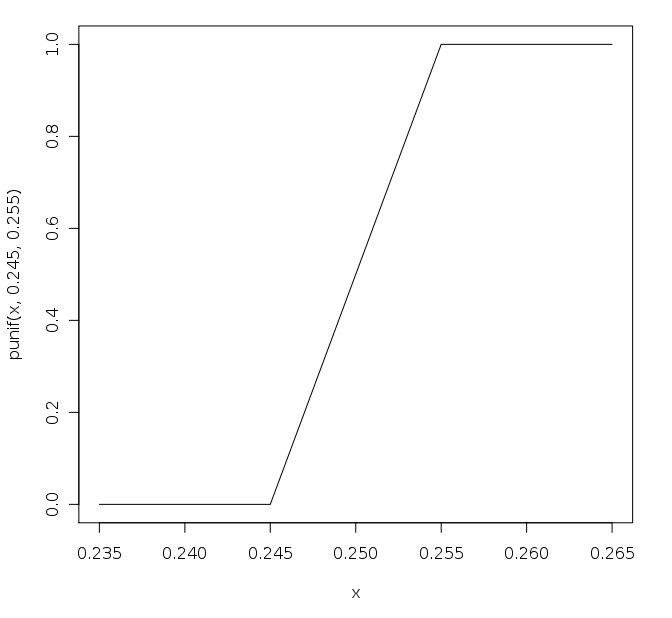
\includegraphics[width=3.3in,height=3.3in]{images/2_1-punif.png}\\
		Funci\'on de densidad de probabilidad:\\
	  	  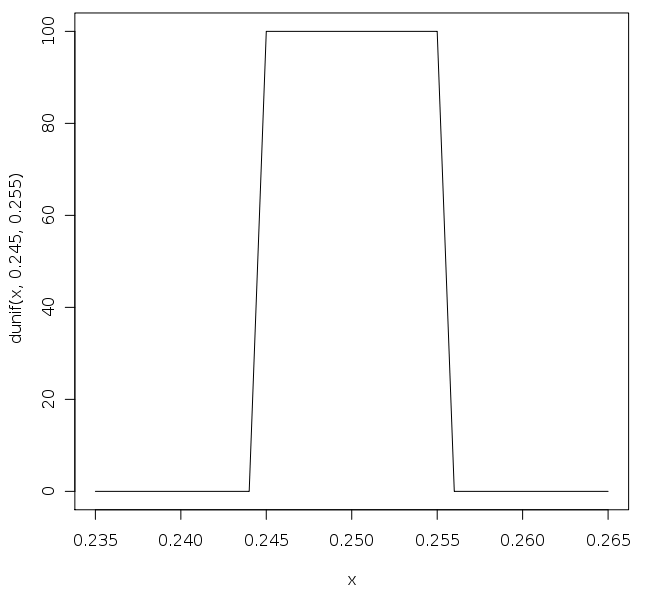
\includegraphics[width=3.3in,height=3.3in]{images/2_1-dunif.png}
	\item Var\'ie el o los valores de los par\'ametros de la distribuci\'on y comente lo observado en los gr\'aficos de la funci\'on de densidad y de distribuci\'on. (2 casos).\\
	\begin{itemize}
		\item Funcion de Densidad\\
			Variando l\'imites (0.240~0.260):\\
		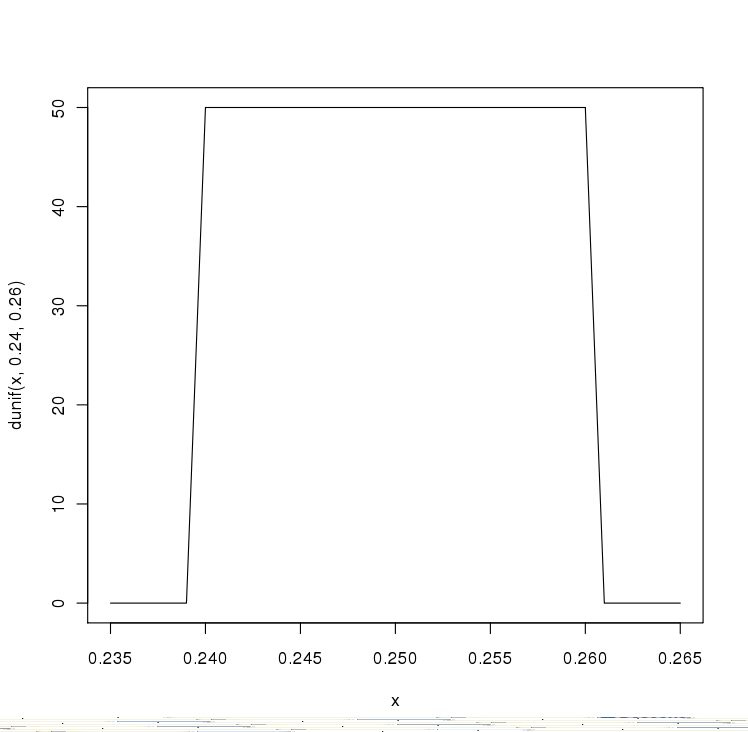
\includegraphics[width=3.3in,height=3.3in]{images/2_1-dunif-variado1.png}\\
			Variando l\'imites (0.235~0.265):\\
		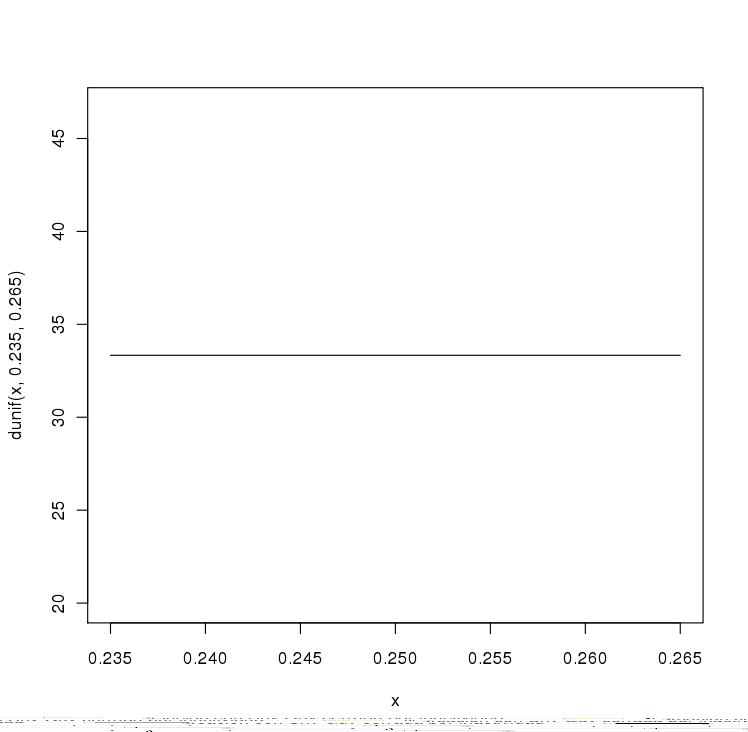
\includegraphics[width=3.3in,height=3.3in]{images/2_1-dunif-variado2.png}\\
		Como podemos ver, al alejarse los limites, tiende a la constante.\\
		\item Funcion de Distribucion\\
                        Variando l\'imites (0.240~0.260):\\
                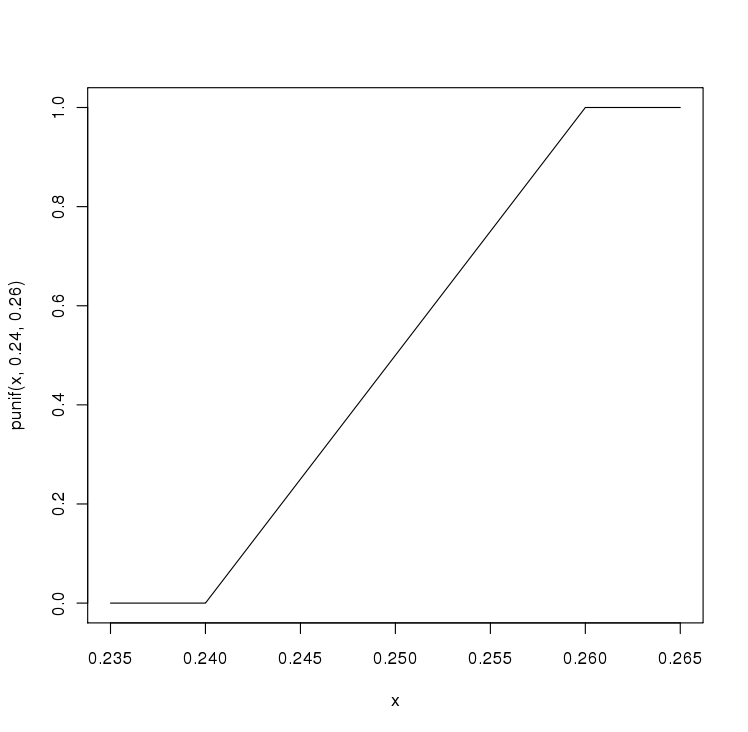
\includegraphics[width=3.3in,height=3.3in]{images/2_1-punif-variado1.png}\\
                        Variando l\'imites (0.235~0.265):\\
                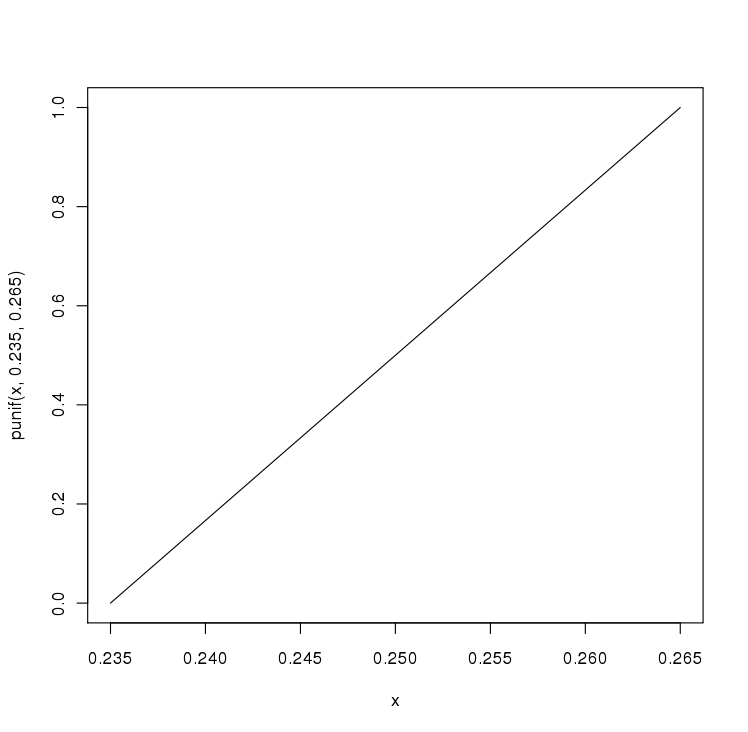
\includegraphics[width=3.3in,height=3.3in]{images/2_1-punif-variado2.png}\\
		Al alejarse los limites, la funcion tiende a una recta.\\

	\end{itemize}

\end{itemize}
